%%
%% This is file `example-1.tex',
%% generated with the docstrip utility.
%%
%% The original source files were:
%%
%% drexel-thesis.dtx  (with options: `example-part')
%% 
%% This is a generated file.
%% 
%% Copyright (C) 2010 W. Trevor King
%% 
%% This file may be distributed and/or modified under the conditions of
%% the LaTeX Project Public License, either version 1.3 of this license
%% or (at your option) any later version.  The latest version of this
%% license is in:
%% 
%%    http://www.latex-project.org/lppl.txt
%% 
%% and version 1.3 or later is part of all distributions of LaTeX version
%% 2003/06/01 or later.
%% 

\chapter{Quasi 2-D and 2.5-D Systems}
Studies of traveling waves have focused on two-dimensional waves that spread parallel to the surface (pia) of the brain \citep{reimer2010}\citep{keane2015}\citep{Townsend2018}\citep{Golomb1997}\citep{Qi2015}. 
This is to be expected as this is the geometry of the system on which they are observed, and \citet{Wilson1973} provide an anatomical argument for focusing on such structure. 

We now expand our study of traveling waves in quasi 1-D minicolumns to two-dimensional topologies.
First we study two-dimensional sheets of neurons extended in the X and Y directions.
As before, we find that our model doesn't support traveling waves in a purely two-dimensional sheet (Z=1) under the model parameters studied.
When we extend the system to a quasi two-dimensional sheet (Z=2) we find traveling waves are evoked by both the background and impulsive stimulus.
We observe several types of waves in our sheets that match those observed in vivo, and demonstrate how model parameters shape the types of waves present in the system.
Our systems exhibit spatiotemporal attractor states, repeating patterns characterized by highly regular inter-spike intervals.
Two identical systems can settle into different attractor states depending on the stimulus applied.

We then further extend our topology to what we term a ``forest'' of minicolumns.
This structure consists of an ensemble of our minicolumns arranged on a grid, with the Z extent less than the X/Y extents.
We find that our forest supports transverse traveling waves in the X/Y plane.

\section{Two-dimensional sheets of neurons}
Traveling waves in two-dimensional neuronal sheets have been studied in the brain \citep{huang2004}\citep{Townsend2018} and in simulation\citep{keane2015}\citep{Spreizer2019}\citep{Bhattacharya2021}.
While one-dimensional waves have only one structure, the additional degree of freedom in two dimensions allows for several categories of waves.
These include circular or ring waves that spread outward from a point, large plane waves that propagate over the entire surface and spiral waves\citep{Huang2010}\citep{Gu2013} that rotate around a central point.
Different types of waves have been associated with different elements of visual stimulus\citep{Benucci2007}.
We find evidence for all these categories of waves in our quasi two-dimensional sheet.

Each sheet consists of neurons placed on a unit grid. 
The X and Y extents are much larger than the Z extent.
We generally use sheets with Z=2 with the exception of one purely two-dimensional example with Z=1.
Neurons are created and connected as described in Methods.
Due to the larger area of regard and the more demanding computational experiments we use periodic boundary conditions in our quasi two-dimensional sheets.
A small example quasi 2-D sheet is shown in Figure \ref{fig:sheet_structure}.
In this small example the periodic boundary conditions are easily seen as multiple diagonals in the connection matrix.

\begin{figure}[!htb]
 \caption{Example small quasi 2-D sheet with dimensions X=10, Y=10, Z=2. The connection parameters are set to $\lambda$=2.5 and C=0.5. 
 a)  Sheet showing connections between neurons as lines colored using a color scale that indicates the connection length. 
 b)  Connection matrix. E-E connections are green, E-I are black and both I-E and I-I  are red. 
 c) The sum of presynaptic weights for each neuron shows the anisotropy of this model, with substantial variation in input strength and sign between the neuron inputs.}
 \label{fig:sheet_structure}
 \subfloat[][]{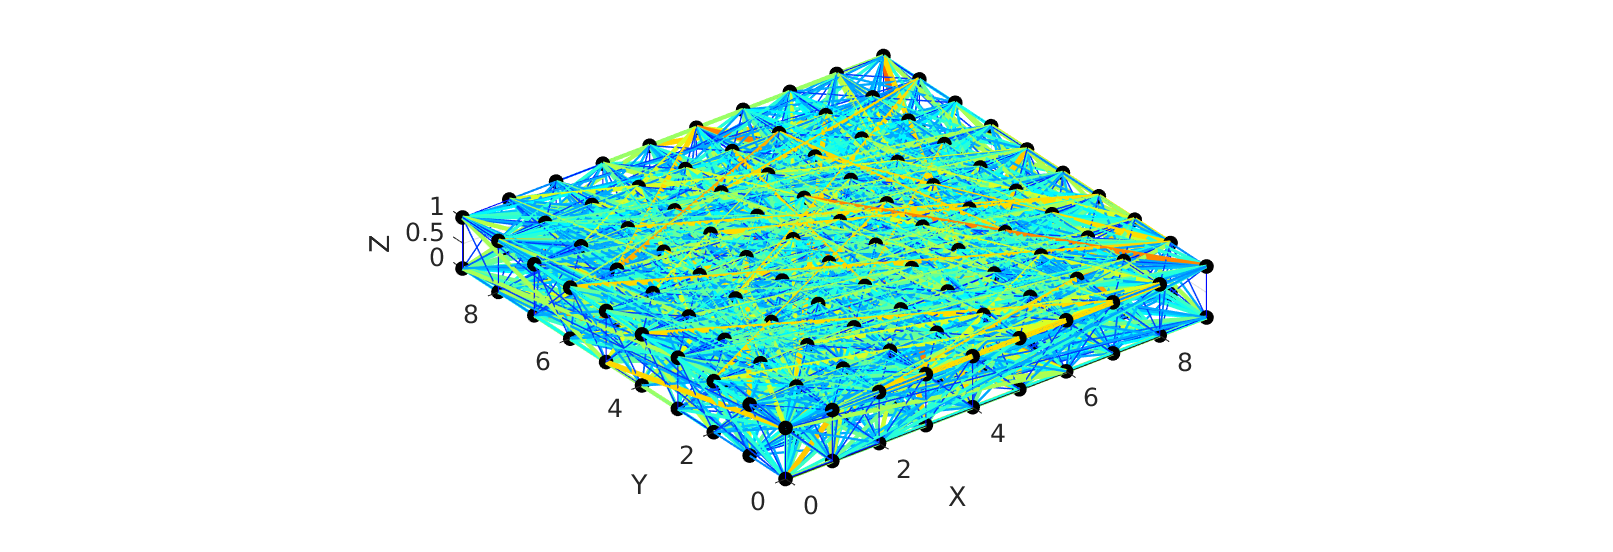
\includegraphics[width=\textwidth]{fig/Sheet_Structure_A}}
 \subfloat[][]{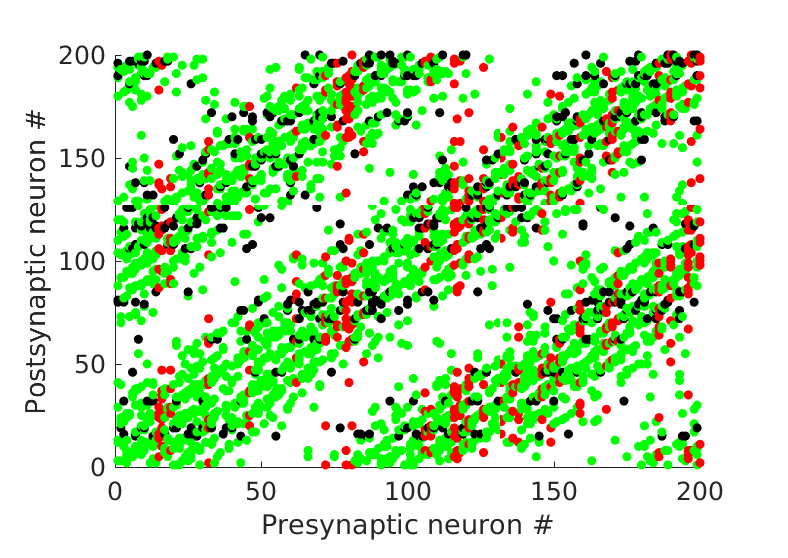
\includegraphics[width=0.4\textwidth]{fig/Sheet_Structure_B}}
 \subfloat[][]{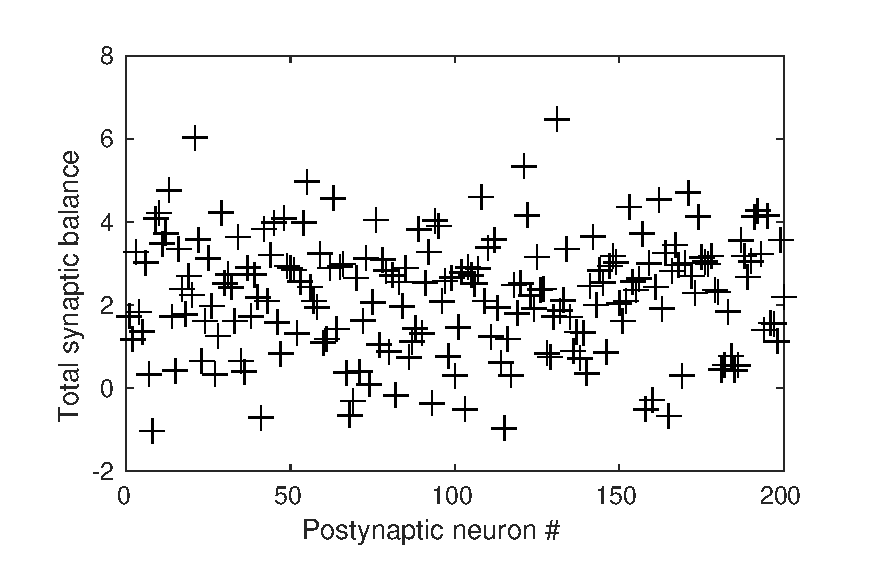
\includegraphics[width=0.4\textwidth]{fig/Sheet_Structure_C}}
\end{figure}

The topology of our sheet combined with our local connectivity rule (eq. \ref{eq:connectivity}) defines the connection distribution of the sheet.
The distribution of post-synaptic connections and delay times are shown in Figure \ref{fig:connection_delay_distrbution_2D} for an example quasi 2-D sheet.
Compared the to minicolumn connection distribution in figure \ref{fig:connection_delay_distrbution} the neurons in our sheet have on average about twice as many connections.
The length of the connections between neurons tends to be longer in the sheet, resulting in a distribution of longer delays 
in figure \ref{fig:connection_delay_distrbution_2D} when compared to figure \ref{fig:connection_delay_distrbution}.
\begin{figure}[!htb]
 \caption{Distribution of (a) number of post-synaptic connections per neuron and (b) delay time. 
          Data was taken from an X=100, Y=100, Z=2 sheet with $\lambda=2.5$, $\kappa=1$ and periodic boundary conditions.  } 
     \subfloat[][]{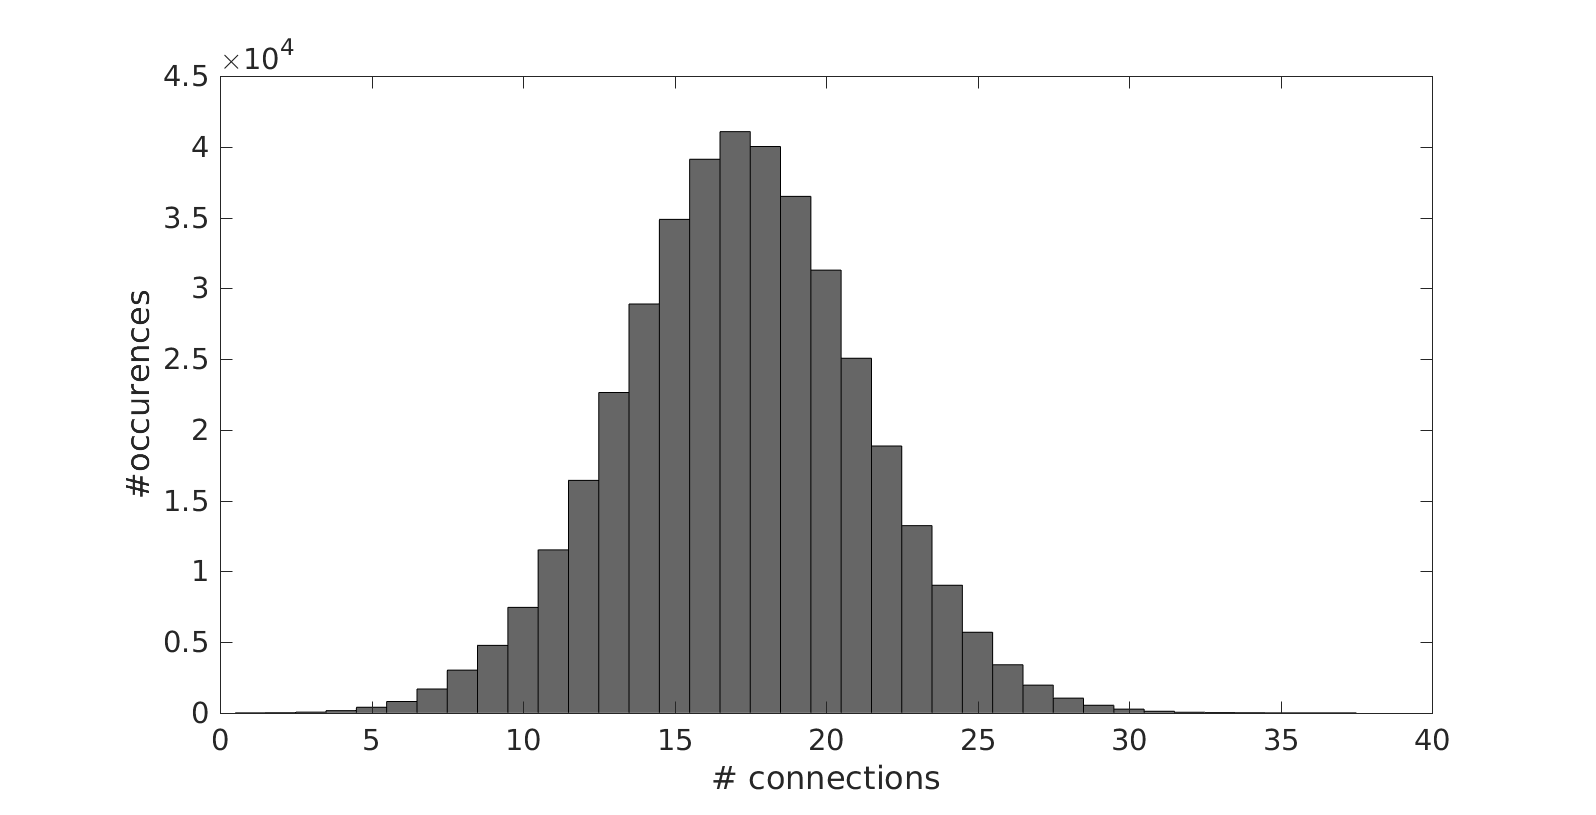
\includegraphics[width=0.6\textwidth]{fig/ConnectionNumberDistribution2D} }
     \subfloat[][]{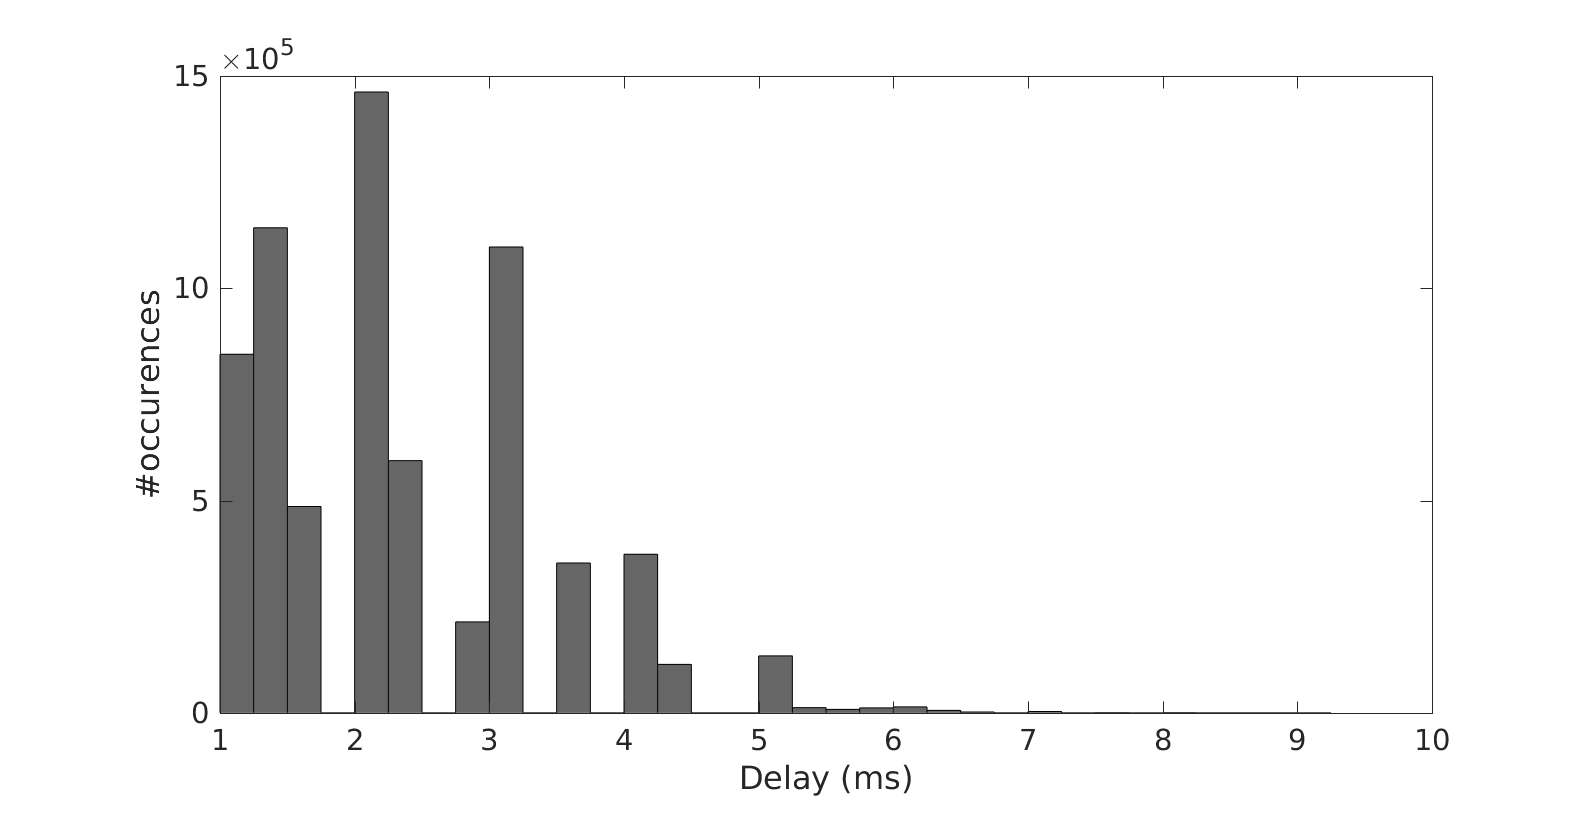
\includegraphics[width=0.6\textwidth]{fig/DelayDistribution2D} }
 \label{fig:connection_delay_distrbution_2D}
\end{figure}
 \FloatBarrier

As we did with our quasi 1-D minicolumn, we first create a purely 2-D sheet of neurons with X=300, Y=300 and Z=1.
Model parameters are fixed at $\Sigma$.
We do not observe traveling waves in this system (Figure \ref{fig:Pure2DRasters_NoWaves}).
\begin{figure}[!htb]
 \caption{Sequential frames showing the average membrane voltage in the X-Y plane.
          The system dimensions are 300x300x1, model parameters are at $\Sigma$. 
	  A 5x5 smoothing filter has been applied to this and all similar figures to enhance the spatiotemporal structure.}
 \label{fig:Pure2DRasters_NoWaves}
 \centering
   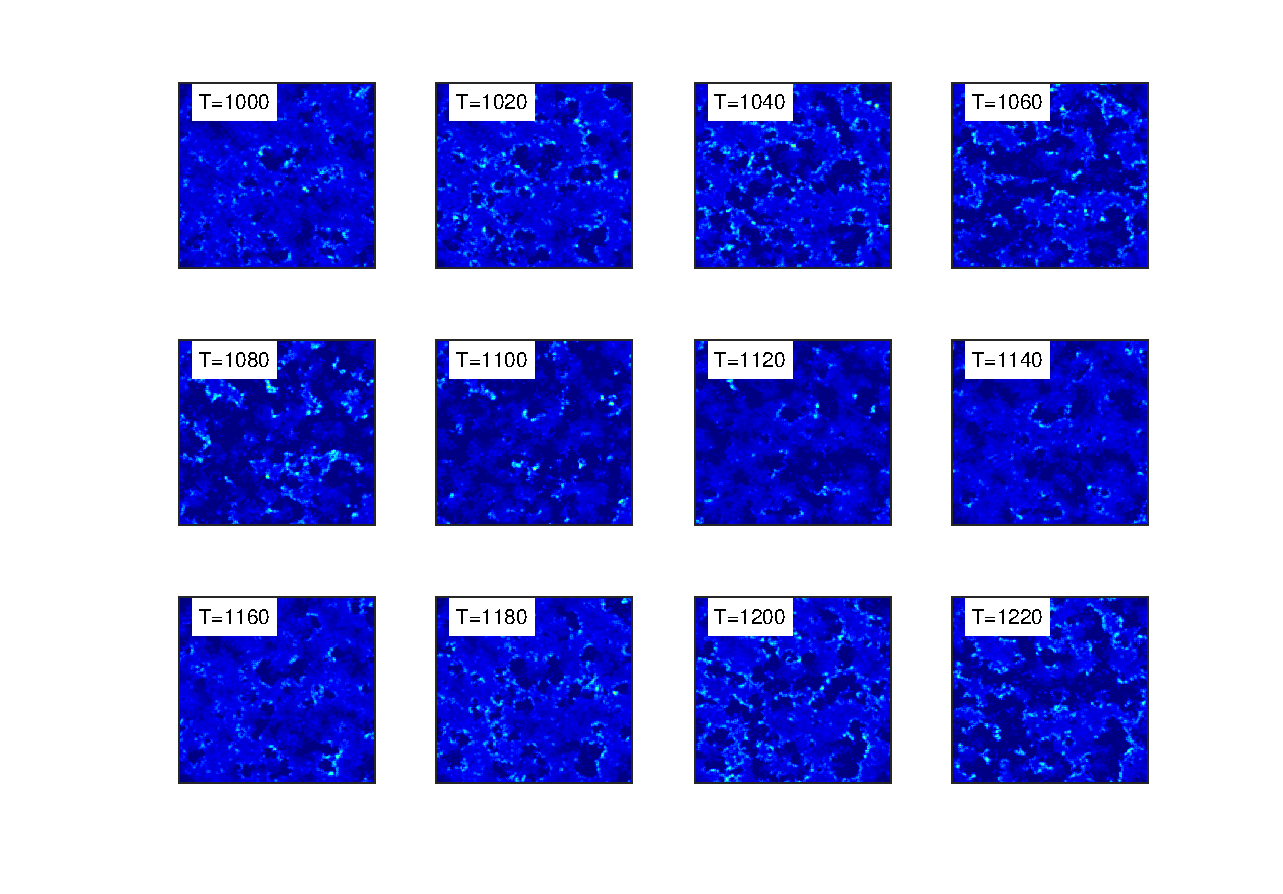
\includegraphics[width=\textwidth]{fig/2D_1LayerNoWaves}
\end{figure}
\FloatBarrier

We do observe a local spatial organization in the activity with nearby neurons tending to fire together.
However this locally coordinated firing activity does not result in traveling waves.
We also see a temporal rhythm with periods of higher and lower activity.
To quantify the temporal rhythm we calculate the inter-spike intervals for every neuron in the simulation.
The distribution of the inter-spike intervals is shown in figure \ref{fig:2D1LayerRhythm}.
\begin{figure}[!htb]
 \caption{The distribution of inter-spike intervals shown on a log scale shows a temporal pattern.
          There is a peak around $180~ms$ with smaller peaks near multiples of $180~ms$.
         }
 \label{fig:2D1LayerRhythm}
 \centering
   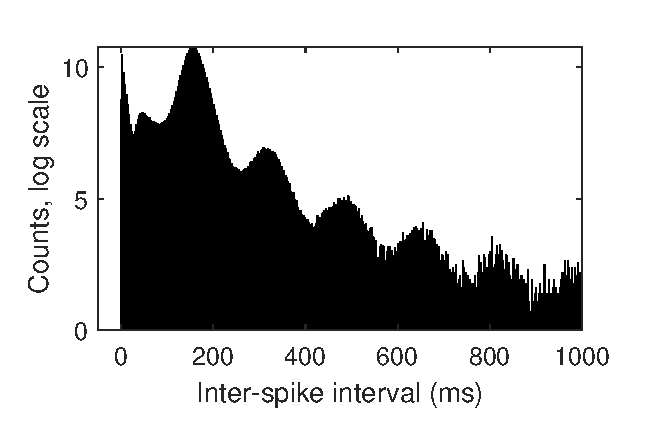
\includegraphics[width=0.6\textwidth]{fig/2D_1Layer_ISI_log}
\end{figure}

\FloatBarrier

We then extend our system to a quasi 2-D sheet with X=300, Y=300 and Z=2.
We now observe traveling wave patterns in the system.
These patterns emerge in spite of the high variability in the neuron types, neuron dynamics and connectivity present in our model.
We can clearly see  circular spreading waves emanating from multiple points within the sheet \ref{fig:2D_waves}.
These types of spreading waves have been observed in vivo\citep{Mohajerani2013} and and in vitro, and can be spontaneously generated or evoked by a stimulus\citep{Stroh2013}.
We observe repetitive patterns, most obviously a large wave emanating from the right side every $250~ms$.
The firing activity in the beginning of the simulation showed more variation, but the large circular wave comes to dominate the firing activity 
in a winner-take-all process due to wave annihilation.
\begin{figure}[!htb]
 \caption{ Wave patterns spreading across the surface of a sheet. 
           The system dimensions 300x300x2, model parameters are at $\Sigma$. 
           Circular spreading waves are evident, especially emanating from a point on the right side of the system.}
 \label{fig:2D_waves}
 \centering
   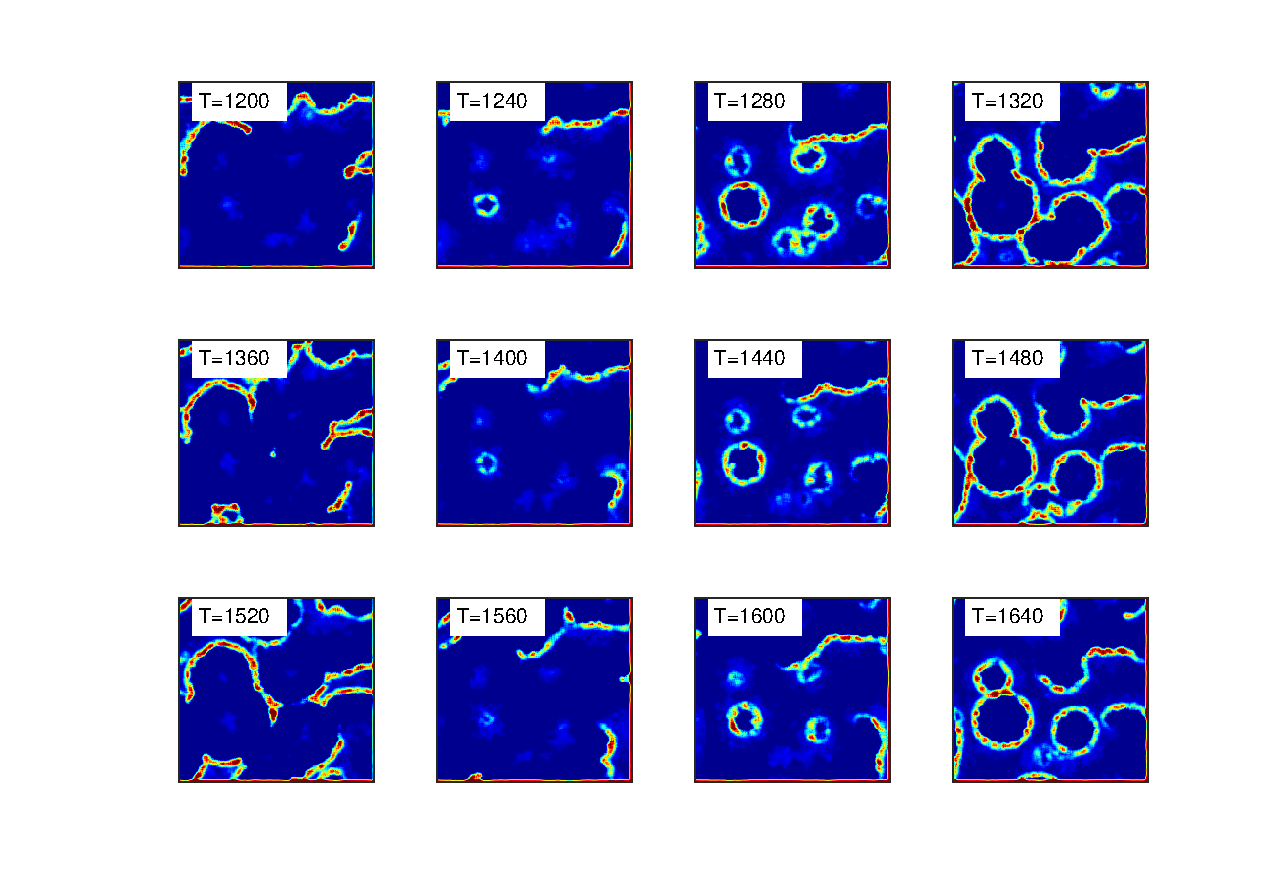
\includegraphics[width=\textwidth]{fig/2DSpreadingWaves_Sigma}
\end{figure}

\FloatBarrier

In some simulations we see the formation of large-scale plane waves across the entire system as seen by \citet{keane2015}.
In their work, plane waves were formed when excitation dominated their neuronal system.
These plane waves seem to form due to the interaction of spreading circular waves.
The formation of plane waves in our system does not seem deterministic, as a different random draw of the uniform background stimulus for the same neuronal system may not exhibit plane waves.
Nonetheless, these results show that plane waves can emerge as a stable pattern in systems of this type even when excitation does not dominate.
\begin{figure}[!htb]
 \caption{ A plane wave front forming from multiple circular spreading waves.
          The system dimensions are 300x300x2, model parameters are at $\Sigma$.
          }
 \label{fig:2D_plane_wave}
 \centering
   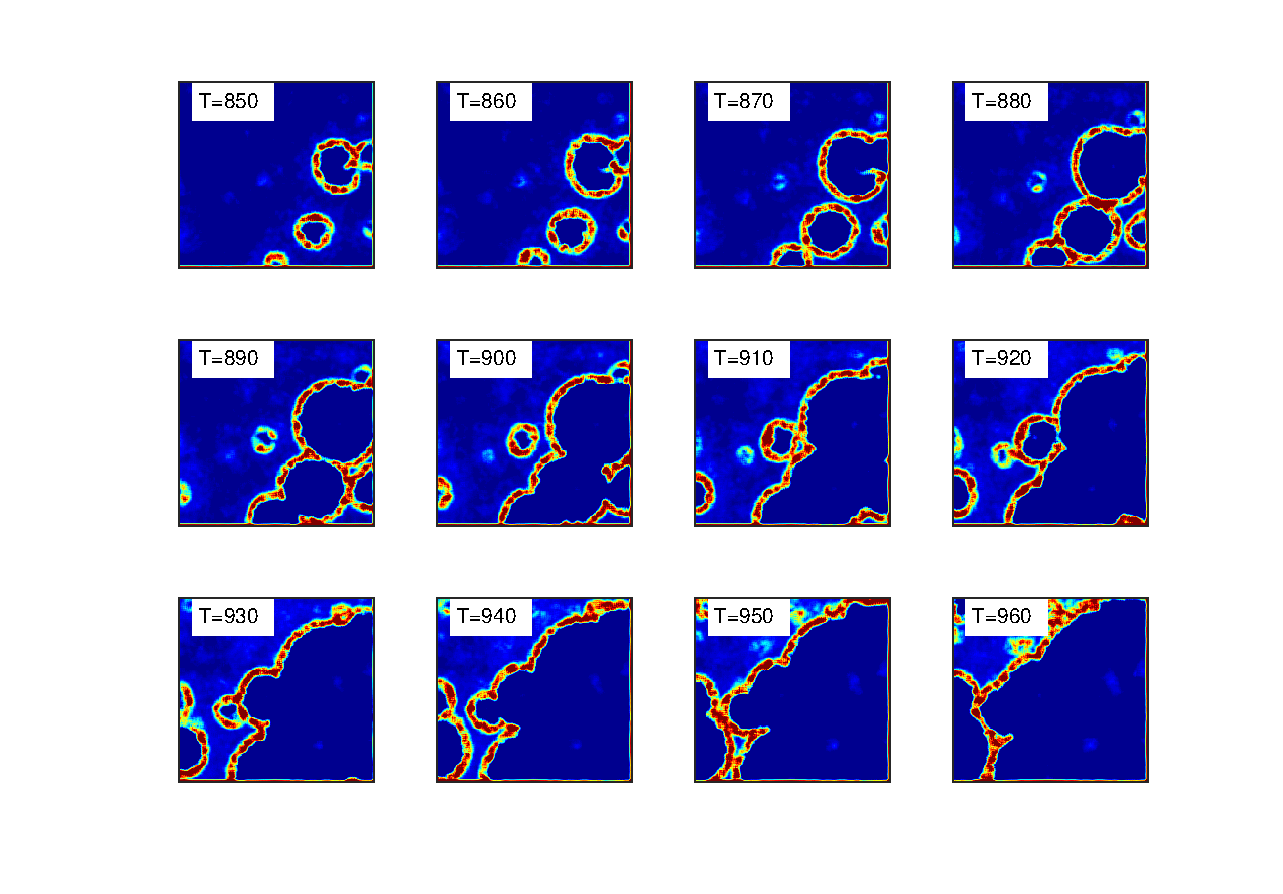
\includegraphics[width=\textwidth]{fig/2DPlaneWave}
\end{figure}
\FloatBarrier

We do not observe spiral waves in our simulations with the model parameters set at $\Sigma$.
With the higher connectivity observed in the sheet (figure \ref{fig:connection_delay_distrbution_2D}) we see circular waves emanating from a point.
Although these waves can combine to form a plane wave structure (figure \ref{fig:2D_plane_wave}), we do not observe spiral wave patterns across many simulations.
We reduce the connection strength K from $K=10$ to $K=6$.
The waves at the lower connection strength are thinner and sparser.
We now observe the formation of spiral wave pattern as seen in figure \ref{fig:2DSpiralWaves}.
\begin{figure}[!htb]
 \caption{ Spiral waves are apparent in the average membrane potential observed in a 2D sheet over time. 
           The system dimensions are 300x300x2. Model parameters are at $\Sigma$ except that $K=6$, $\kappa=0.1$.
           }
 \label{fig:2DSpiralWaves}
 \centering
   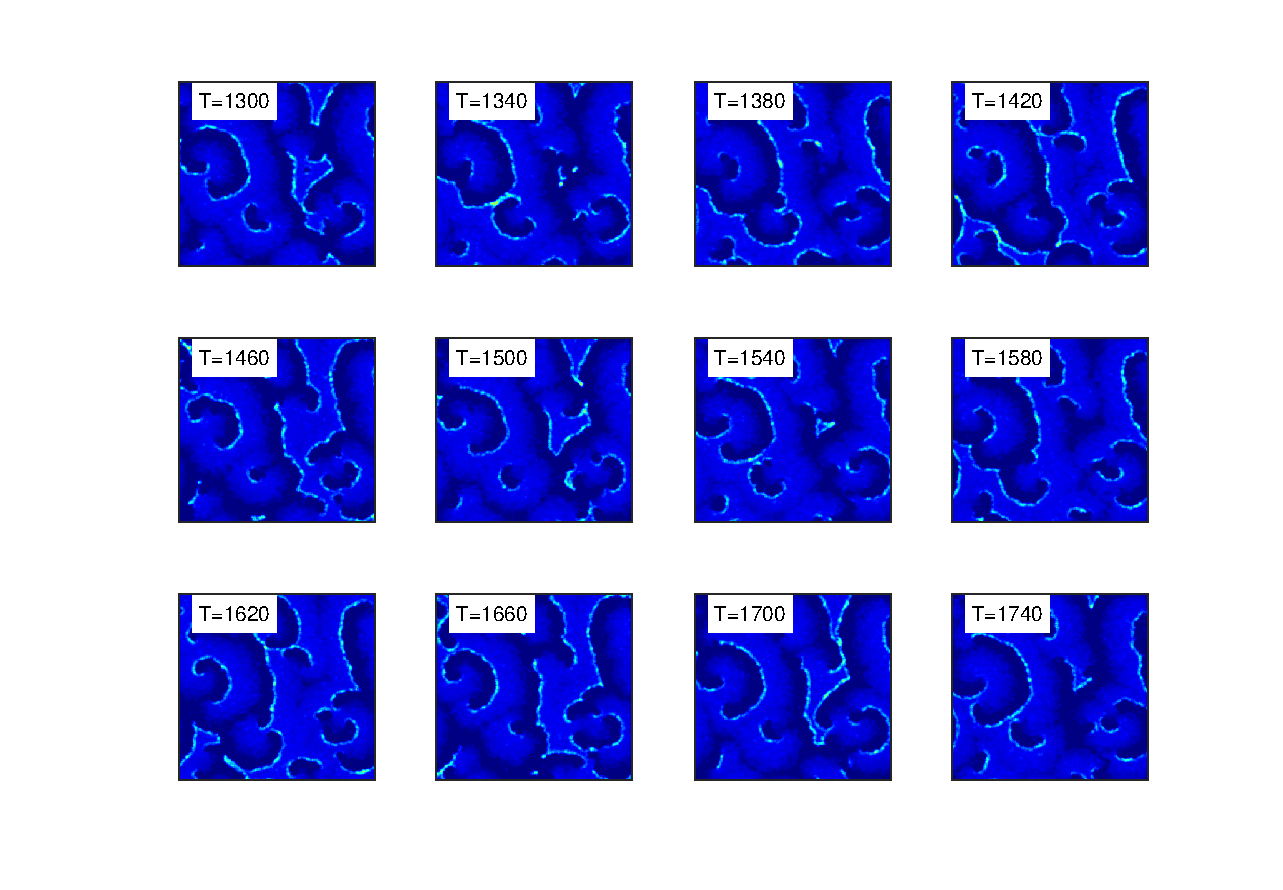
\includegraphics[width=\textwidth]{fig/SpiralWaves2D_K6_kappa0p1_M4}
\end{figure}
\FloatBarrier

\citet{Huang2010} provide the observation that a plane wave with limited extents can generate a spiral wave pattern.
The firing activity at the edge of the plane wave will spread in directions that are not parallel to the plane wave propagation.
We observe similar behavior when the propagation of a circular spreading wave is not isotropic.
In this case we can see spiral waves shed from both edges of the circular wave as seen in figure \ref{fig:2DHeartWaves}.
We term these 'heart' waves.
\begin{figure}[!htb]
 \caption{ Spiral 'heart' waves are apparent in the average membrane potential observed in a 2D sheet over time. 
           The sheet is 200x200x2 with periodic boundary conditions, $K=6$, $\kappa=0.1$.
           }
 \label{fig:2DHeartWaves}
 \centering
   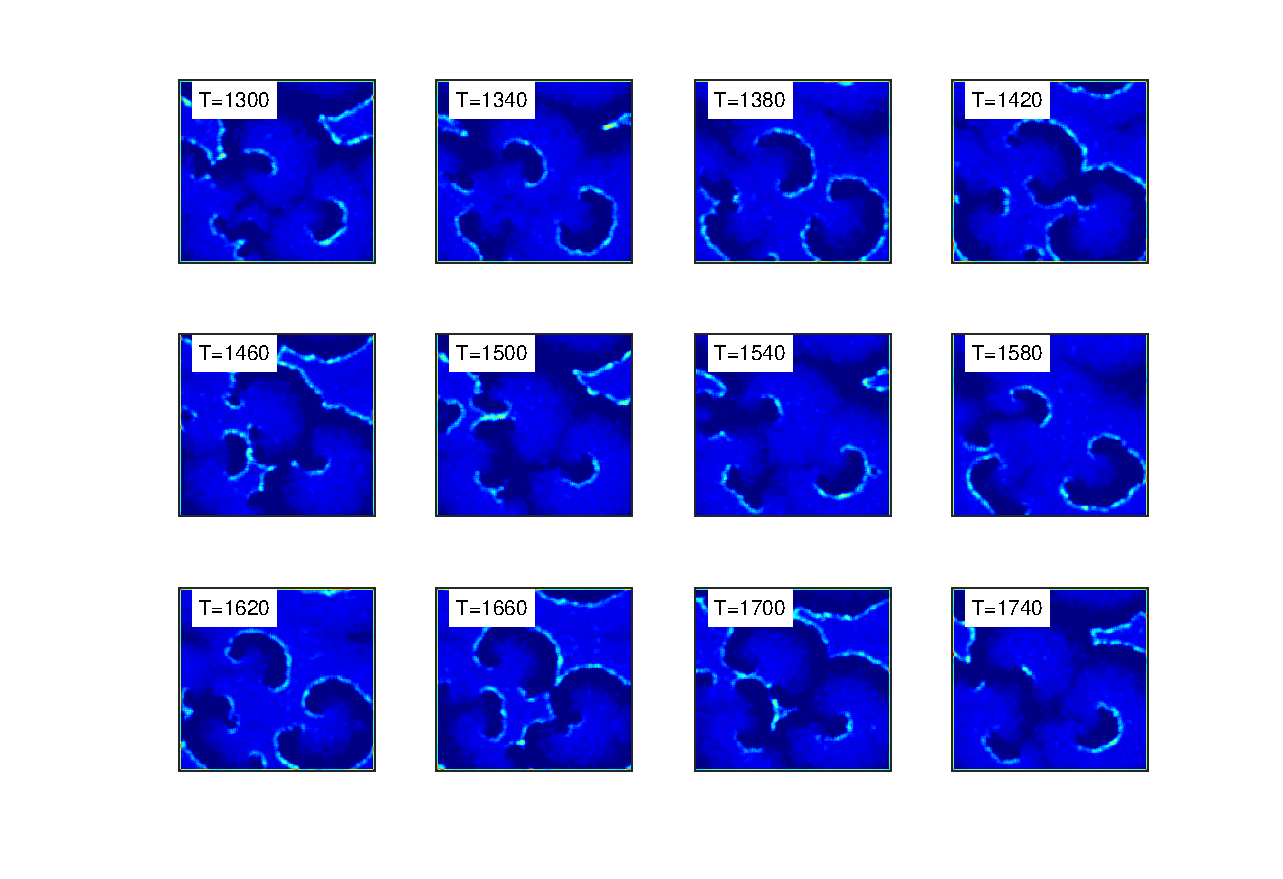
\includegraphics[width=\textwidth]{fig/2DSpiralWaves_HeartWaves}
\end{figure}
\FloatBarrier

We further examine the transition from spreading waves to spiral waves as connection strength decreases.
We hypothesize that the lower connection strength creates anisotropy that can disrupt a spreading wave propagation, resulting the heart and spiral patterns. 
We demonstrate this using a 100x100x2 sheet with a step stimulus as described in section \ref{sec:wave_speed_method}.
The stimulus is applied to the neurons at the center of the sheet at $t=0$ and generates waves that radiate outward.
The smaller system size is valid as we are creating a single controlled wave at the center of the system.
Examples of the waves in the system are shown in Figure \ref{fig:2DWaveTransition}a and \ref{fig:2DWaveTransition}b.

We wish to determine whether a given experiment produced a spreading wave or spiral wave.
To distinguish between the wave types we calculate the center of mass of the spikes that occur in a $5~ms$ window:
\begin{align}
 CoM_x &= \frac{1}{N_{spikes}}\Sigma_{i=1}^{N_{spikes}} X_i\\
 CoM_y &= \frac{1}{N_{spikes}}\Sigma_{i=1}^{N_{spikes}} Y_i
\end{align}
where $X$ and $Y$ are the X and Y locations of the spikes w.r.t to center of the sheet, and $N_{spikes}$ is the total number of spikes that occur in the $5~ms$ observation.
We then calculate the center of mass offset as $d_{CoM}=\sqrt{CoM_x^2 + CoM_y^2}$.
The spreading waves have a low $d_{CoM}$ due to their high symmetry, while the spiral waves have a higher $d_{CoM}$.
We see in Figure \ref{fig:2DWaveTransition}c that he $d_{CoM}$ clearly shows the transition from spiral waves to spreading waves as $K$ increases.
\begin{figure}[!htb]
 \caption{Transition between spiral and spreading waves as $K$ increases.
          a) Spike raster plot showing a spiral wave in a sheet with $K=9.5$. The center of mass is displaced almost 22 units from the center at $t=100$ indicating the asymmetry of the wave.
          b) Spike raster plot showing a spreading wave in a sheet with $K=10.5$. The center of mass is displaced only 2.5 units due to the high symmetry of the wave.
          c) The system undergoes a transition from asymmetric spiral waves to symmetric spreading waves as the connection strength parameter $K$ increases.
          } 
     \subfloat[][]{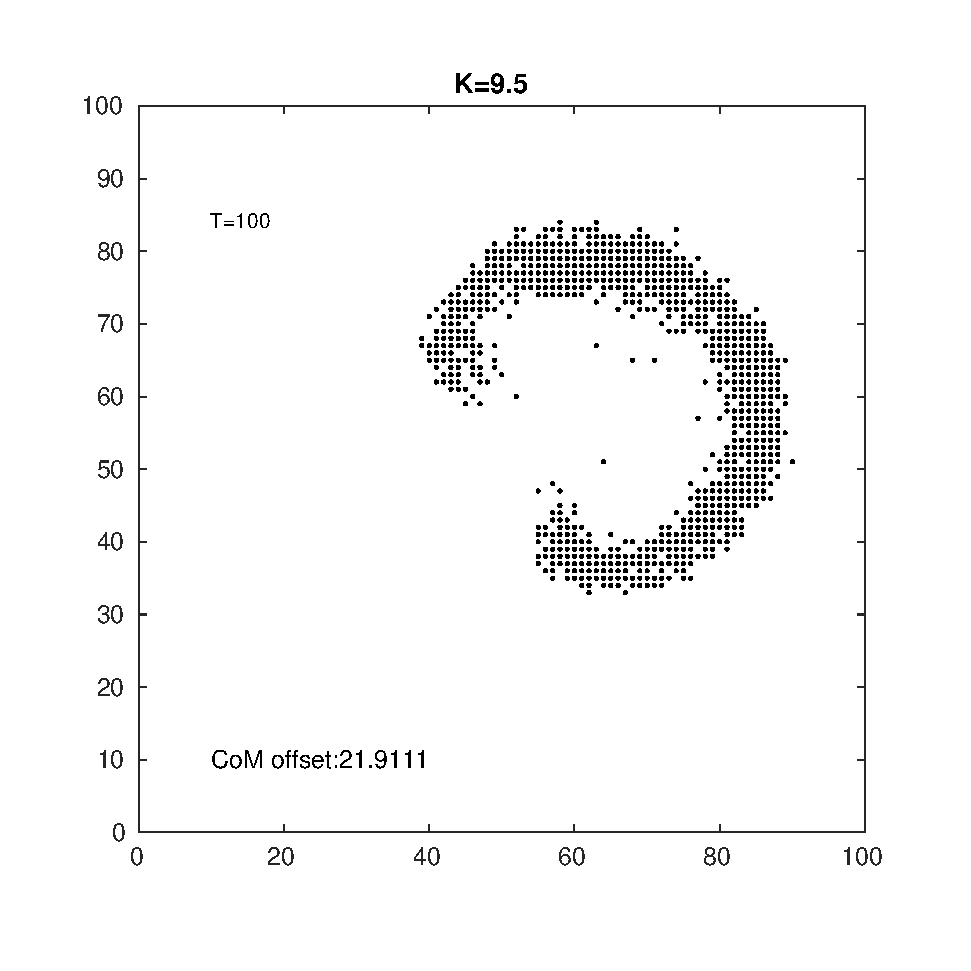
\includegraphics[width=0.45\textwidth]{fig/CoM_Example_K_9p5} }
     \subfloat[][]{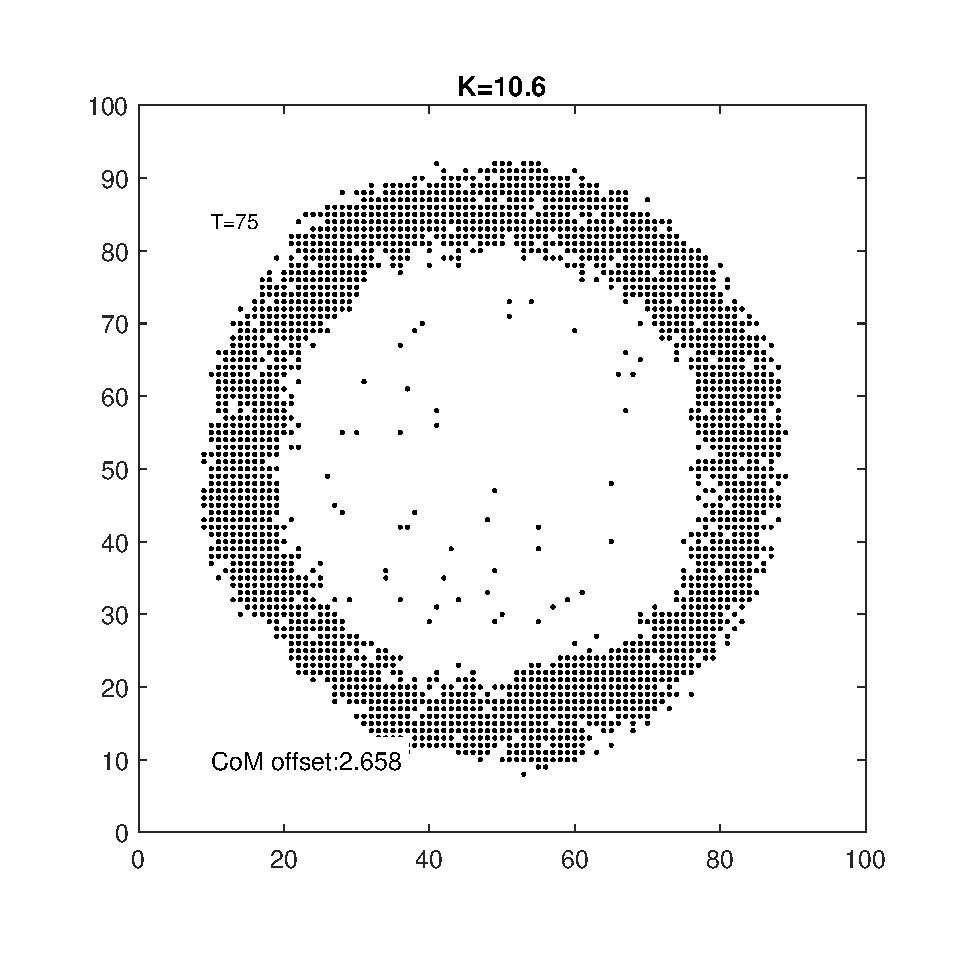
\includegraphics[width=0.45\textwidth]{fig/CoM_Example_K_10p5} }
     \subfloat[][]{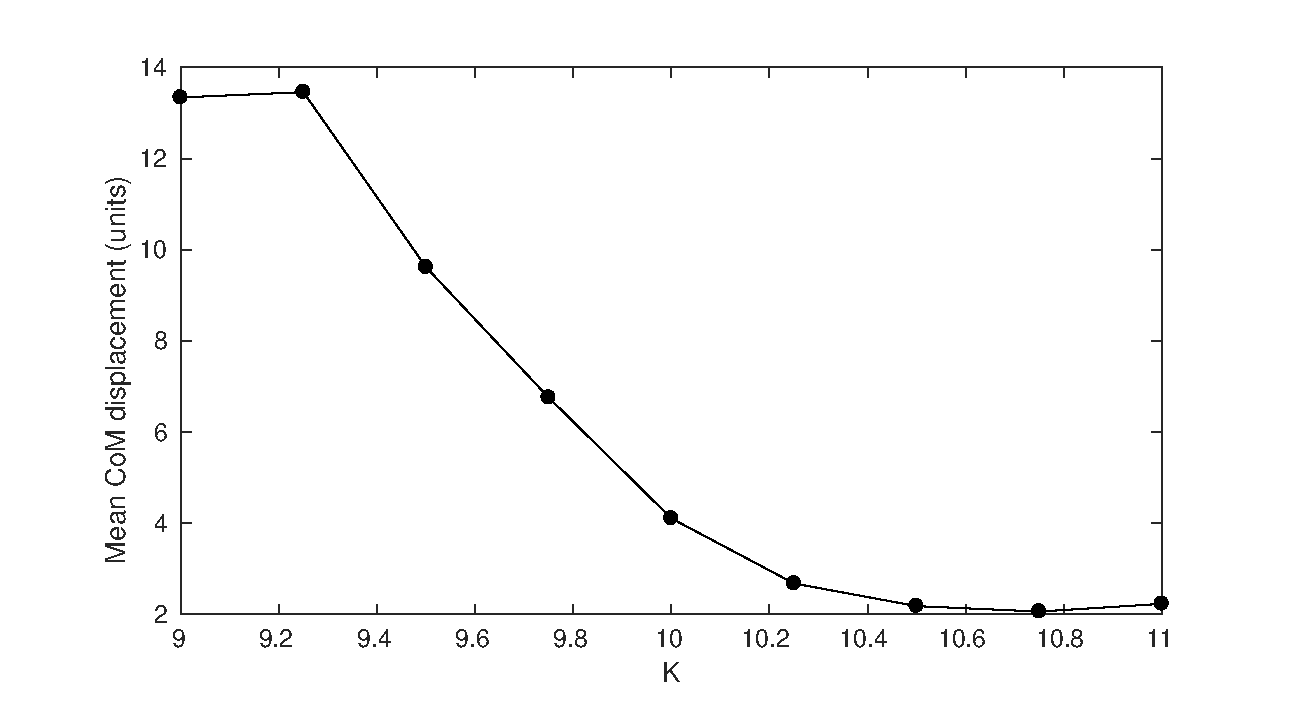
\includegraphics[width=0.75\textwidth]{fig/2DWaveTypeTransition} }
 \label{fig:2DWaveTransition}
\end{figure}
 \FloatBarrier

The waves in our simulations appear to create spatiotemporal patterns that repeat at some regular interval.
This is in contrast to \citet{keane2015} who proposed traveling waves in 2-D sheets to explain why individual spike timing is highly irregular 
but membrane potential fluctuations can be correlated.
To compare our system to \citet{keane2015} we calculate the coefficient of variation of the inter-spike intervals for the spiral wave experiment:

We examine the coefficient of variation and spike count cross-correlation for the simulation show in figure \ref{fig:2DSpiralWaves}.
As seen in figure \ref{fig:2DSpiralWave_SpikeTiming} the typical coefficient of variation is closer to 0 indicating highly regular firing.
This is in contrast with the simulated results in \citet{keane2015} who observed highly irregular spiking in the individual neurons.
Our observation is qualitatively in agreement with voltage-sensitive dye experiments where any given pixel of the VSD image shows highly repetitive fluctuations (\citet{Huang2010} figure 1, \citet{huang2004} figure 2). 
The spike count correlation, when plotted as a function of the distance between neurons, shows that neurons that are closer together have more correlated activity.
This is in agreement with both simulated and observed traveling wave experiments.

\begin{figure}[!htb]
 \caption{Spike timing characterization of the spiral waves seen in figure \ref{fig:2DSpiralWaves}.
          a) The spike raster from a small number of neurons show regular spike events that correspond to passing waves.
          b) The histogram of all inter-spike intervals shows a peak $200~ms$ corresponding to the wave repetition rate. The peak near 0 is due to neurons firing several times when a wave passes. 
          c) The distribution of the coefficient of variation (eq. \ref{eq:cv}) confirms the regular spiking behavior as most of the CV values are near 0 (perfectly regular).
          d) The average correlation coefficient as a function of distance (\ref{eq:cross_correlation}) shows that the firing times of nearby neurons are highly correlated due to the wave structure.
          } 
     \subfloat[][]{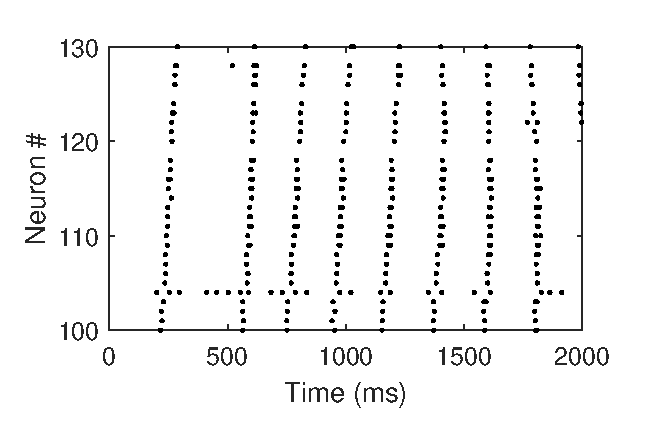
\includegraphics[width=0.48\textwidth]{fig/2DSpiralWaves_CorrelationRasterPlot} }
     \subfloat[][]{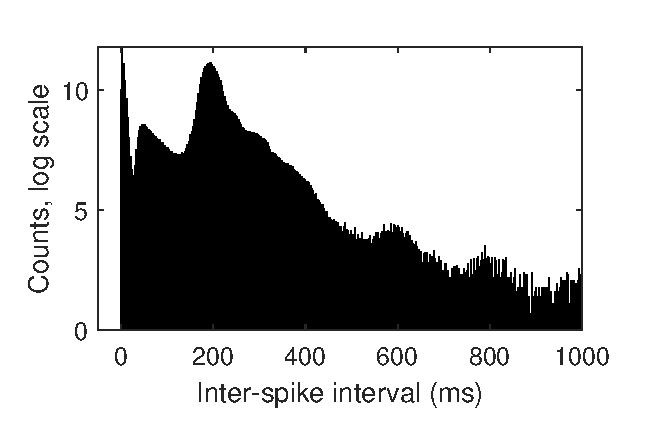
\includegraphics[width=0.48\textwidth]{fig/2DSpiralWaves_ISI_log} }
     \subfloat[][]{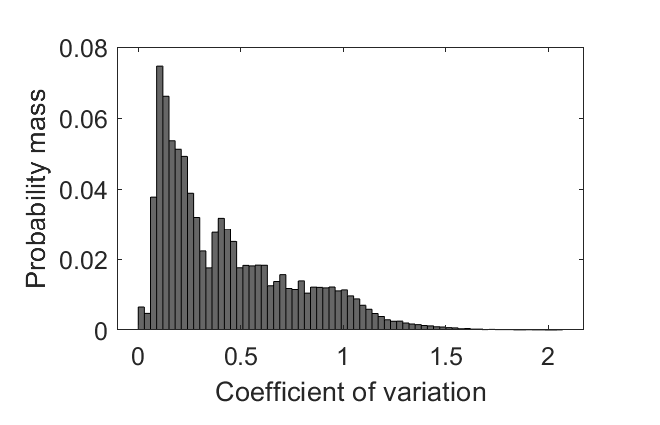
\includegraphics[width=0.48\textwidth]{fig/2DSpiralWaves_CVDist} }
     \subfloat[][]{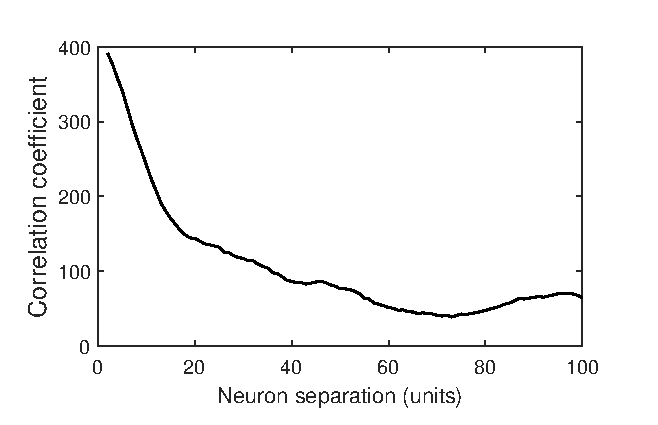
\includegraphics[width=0.48\textwidth]{fig/2DSpiralWaves_CorrelationCoefficient} }
 \label{fig:2DSpiralWave_SpikeTiming}
\end{figure}
 \FloatBarrier
 
This indicates that our 2D sheets exhibit spatiotemporal patterns that are both highly complex and yet repetitive over long time scales.
We consider a complex but repeating pattern as a dynamical attractor of the system.
To understand if the same system has multiple attractor states we compare multiple simulations of an identical system under different random stimulus.
\begin{figure}[!htb]
 \caption{ Another trial of the identical system from Figure \ref{fig:2DSpiralWaves}, but with a different random draw of the stimulus.
           The qualitative behavior is similar but the specific spatiotemporal pattern is clearly different.}
 \label{fig:2DSpiralWaves_SecondTrial}
 \centering
   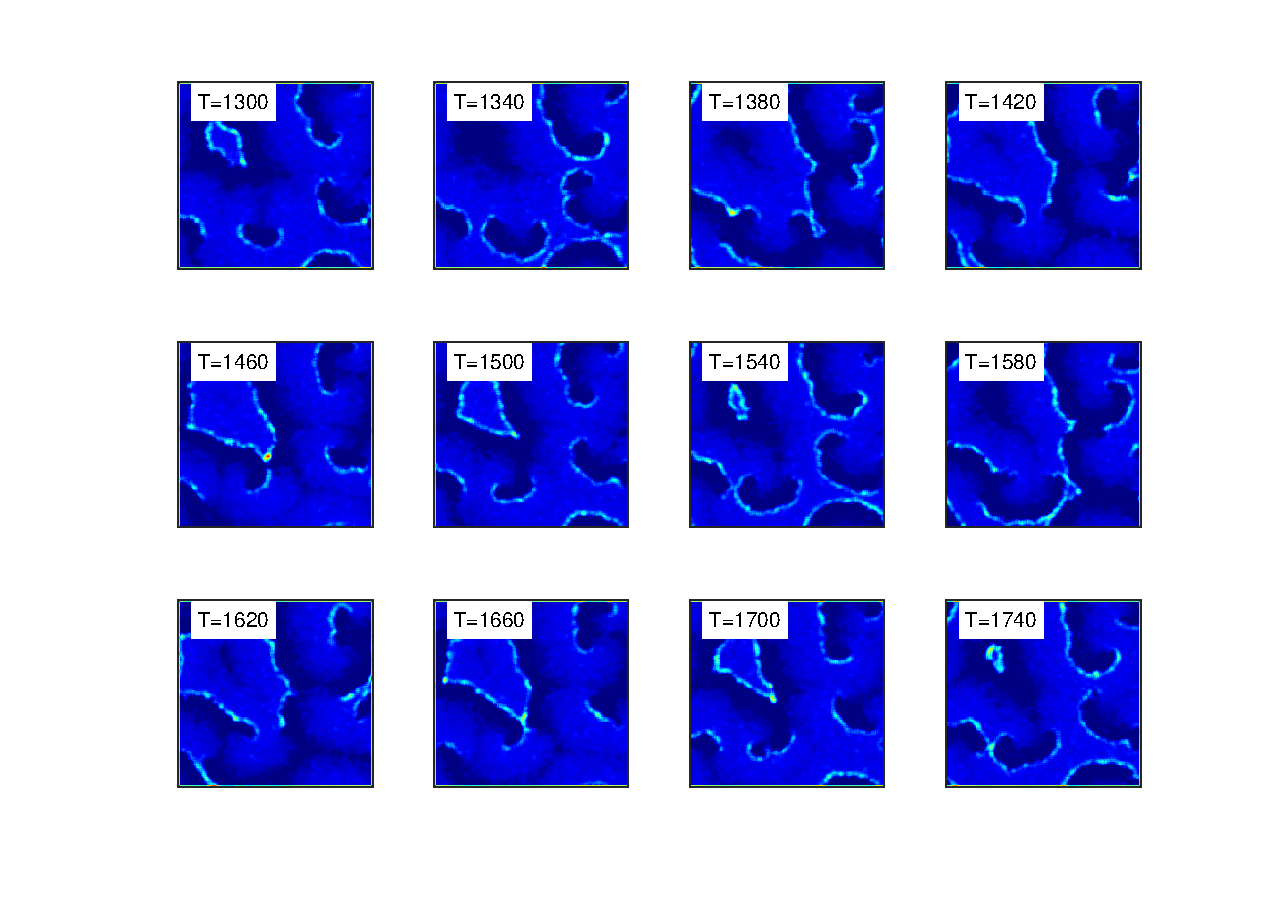
\includegraphics[width=\textwidth]{fig/SpiralWaves2D_K6_kappa0p1_M4_SecondTrial}
\end{figure}
\FloatBarrier

The traveling wave mechanism in the locally connected two dimensional sheet is the same as the locally connected one dimensional minicolumn.
We therefore expect similar traveling wave speeds, with the model parameters playing the same role as in the one dimensional minicolumn.
To measure speed in the sheet we extend the approach taken for the minicolumn by using an impulsive stimulus (equation ).
We use open boundary conditions when measuring wave speed in the two dimensional sheet.
We again find that we need to increase the connection strength $K$ when using an impulsive stimulus instead of a uniform background stimulus.
The neurons in the lower left corner near X=0, Y=0 are stimulated with a constant current for the first 10 milliseconds of the simulation.
This induces a circular spreading wave that spans the sheet as shown in figure \ref{fig:2DWaveSpeedRaster}.
The wave propagates isotropically with the same speed along both the X and Y axes.
The wave spans $100$ units in $192~ms$ for a speed of $0.52$ units/millisecond.
This is faster than the measured wave speed of $0.38$ units/millisecond in the minicolumn with the same model parameters.
As seen in figure \ref{fig:delay_topology} increasing the physical extents of our system increases the 
connectivity (figure \ref{fig:connection_delay_distrbution_2D}) leading to faster wave speeds.
\begin{figure}[!htb]
 \caption{ 2-D spike raster plots showing a single traveling wave.
           The sheet is 100x100x2 with model parameters at $\Sigma_v$ and $\kappa=1.0$.
           }
 \label{fig:2DWaveSpeedRaster}
 \centering
   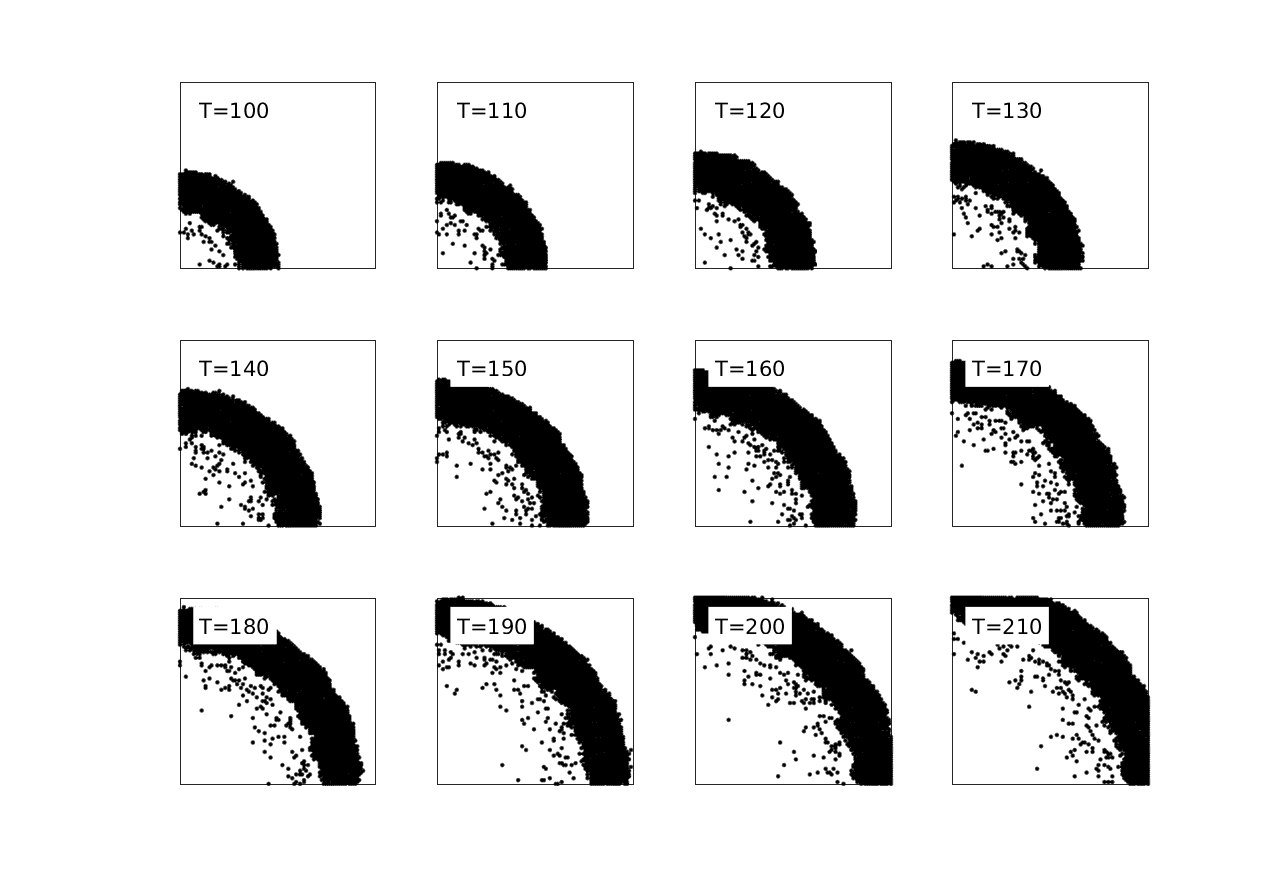
\includegraphics[width=\textwidth]{fig/2DWaveRasters_WaveSpeedExample}
\end{figure}
\FloatBarrier

The wave speed in our sheet depends on $\kappa$ (figure \ref{fig:2DWavePaceKappa}).
The slope of the linear fit matches the one-dimensional system (figure \ref{fig:delay_speed}). 
The lower y-intercept point in the sheet compared to the minicolumn indicates the lower pace (higher speed) due to the higher connectivity in the sheet.
\begin{figure}[!htb]
 \caption{ The pace of the wave depends linearly on $\kappa$.
           }
 \label{fig:2DWavePaceKappa}
 \centering
   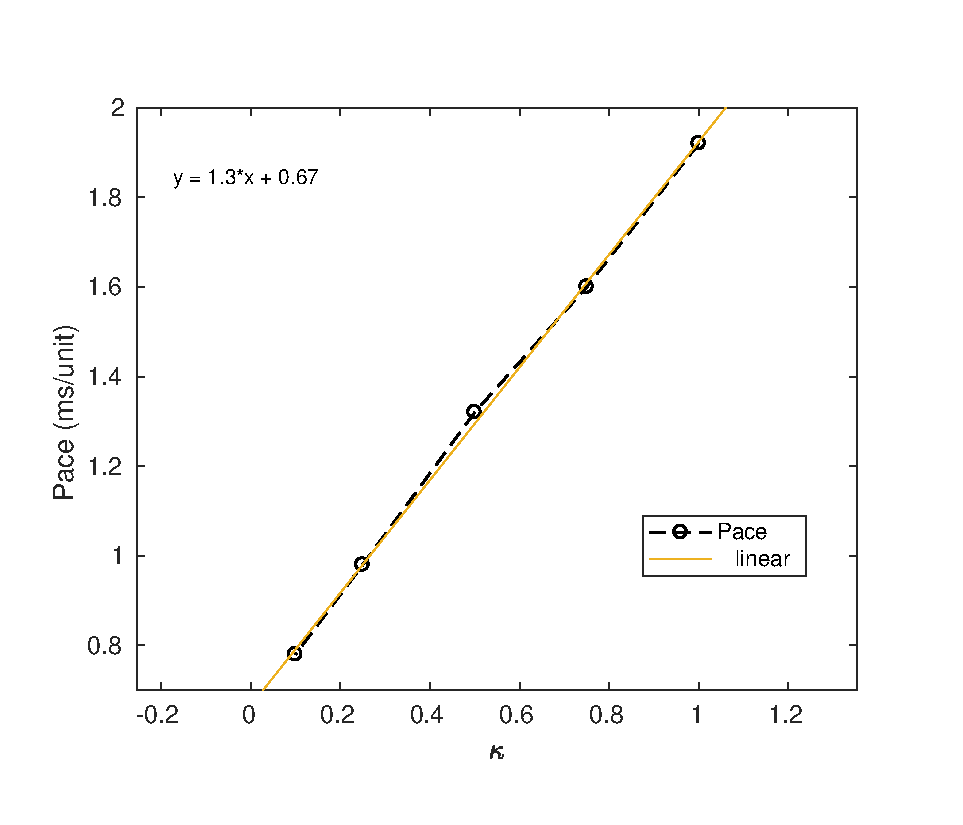
\includegraphics[width=0.5\textwidth]{fig/2DWavePace_Kappa}
\end{figure}
\FloatBarrier


\section{Forests of minicolumns}
The cortex has a laminar vertical organization consisting of six layers \citep{Strominger2012}.
In the visual cortex spontaneous and stimulus-evoked activity can be initiated in different layers\citep{Sakata2009}.
The minicolumn structures observed in the cortex are oriented perpendicular to the layers \citep{cruz2000}\citep{cruz2005}.
We extend our previous quasi one-dimensional and quasi two-dimensional systems to a ``forest'' of minicolumns.
Each individual minicolumn has dimensions 2x2x10.
The foresst of minicolumns are ensembles of 400 or 2500 minicolumns arranged in a 20x20 or 50x50 pattern.
A small example forest is shown in Figure \ref{fig:forest_structure}.
\begin{figure}[!htb]
 \caption{ Example forest of 16 minicolumns arranged in a 4x4 grid, with $1\lambda$ spacing between the closest neurons of any two minicolumns. 
           Each minicolumn has dimensions X=2, Y=2, Z=5. The connection parameters are $\lambda$=2.5 and C=0.5. 
           The connections between neurons as lines colored using a color scale that indicates the connection length. }
 \label{fig:forest_structure}
 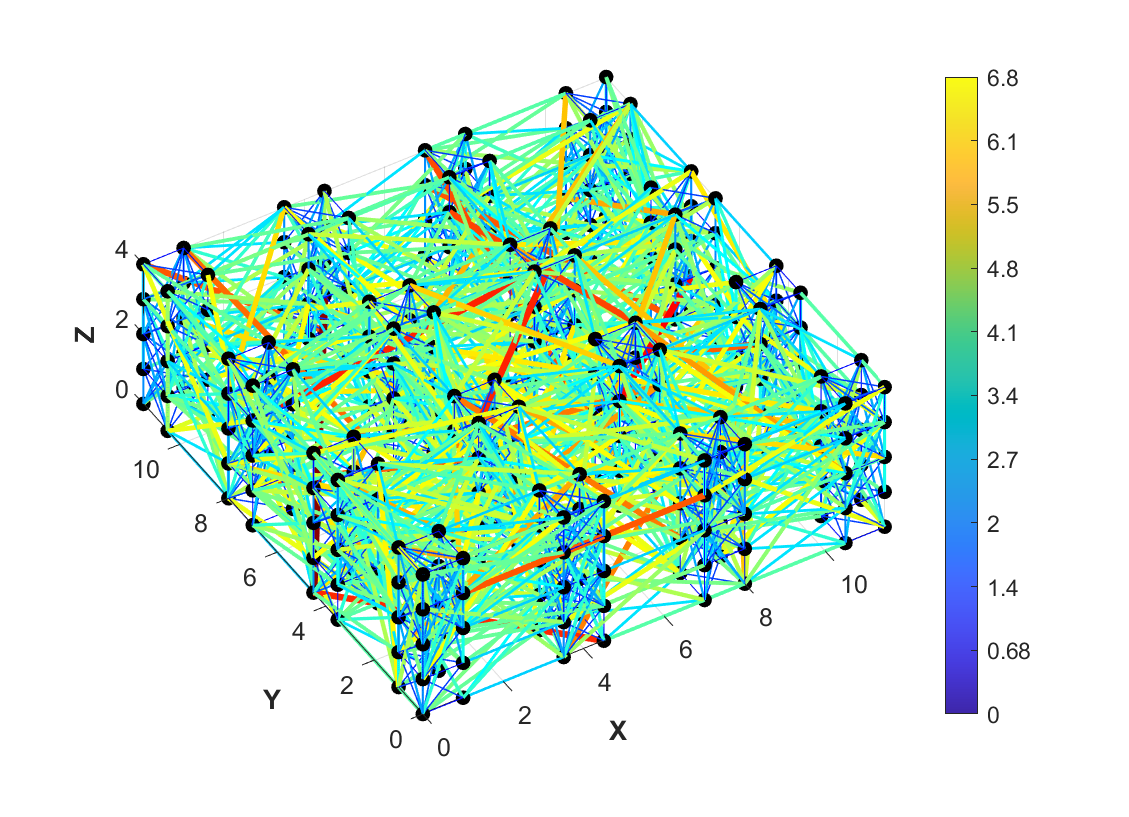
\includegraphics[width=0.75\textwidth]{fig/Forest_Structure_A}
\end{figure}
\FloatBarrier

The distribution of post-synaptic connections and delay times are shown in Figure \ref{fig:connection_delay_distrbution_forest} for an example forest.
The average number of connections appears normally distributed with the mean  number of connections around 7.
This is comparable to the distribution in a single minicolumn (figure \ref{fig:connection_delay_distrbution}),
indicating that the intra-column connectivity is dominant. 
This is also visually apparent in figure \ref{fig:forest_structure} where the connections between microcolumns are sparse compared to the intra-column connections.
\begin{figure}[!htb]
 \caption{Distribution of (a) number of post-synaptic connections per neuron and (b) delay time. Data was taken from a 20x20 forest of 400 minicolumns, each minicolumn 2x2x10, $\lambda=2.5$, $\kappa=1$.  } 
     \subfloat[][]{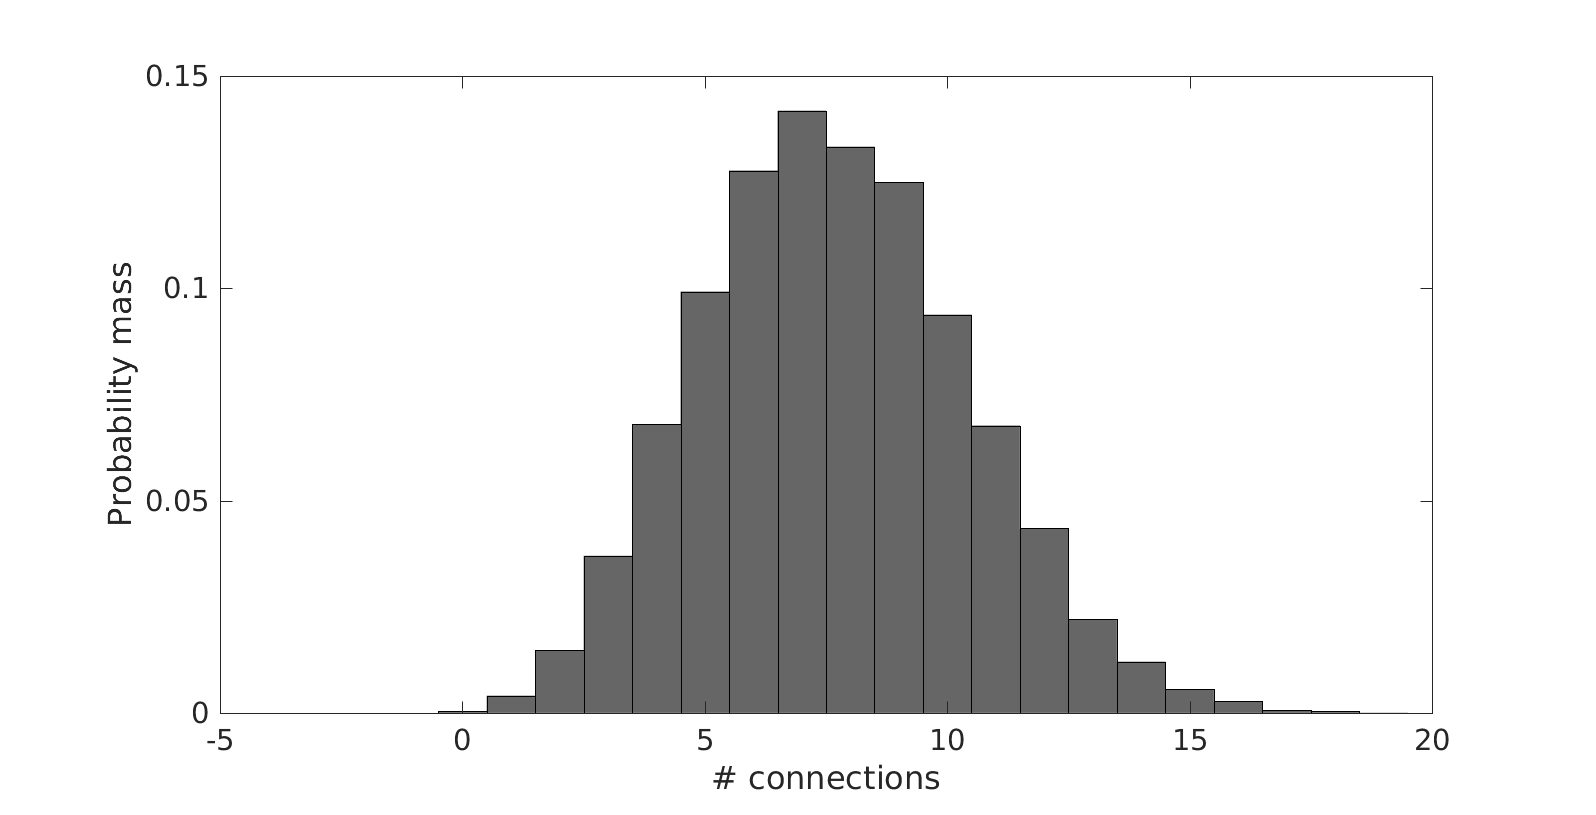
\includegraphics[width=0.6\textwidth]{fig/ConnectionNumberDistributionForest} }
     \subfloat[][]{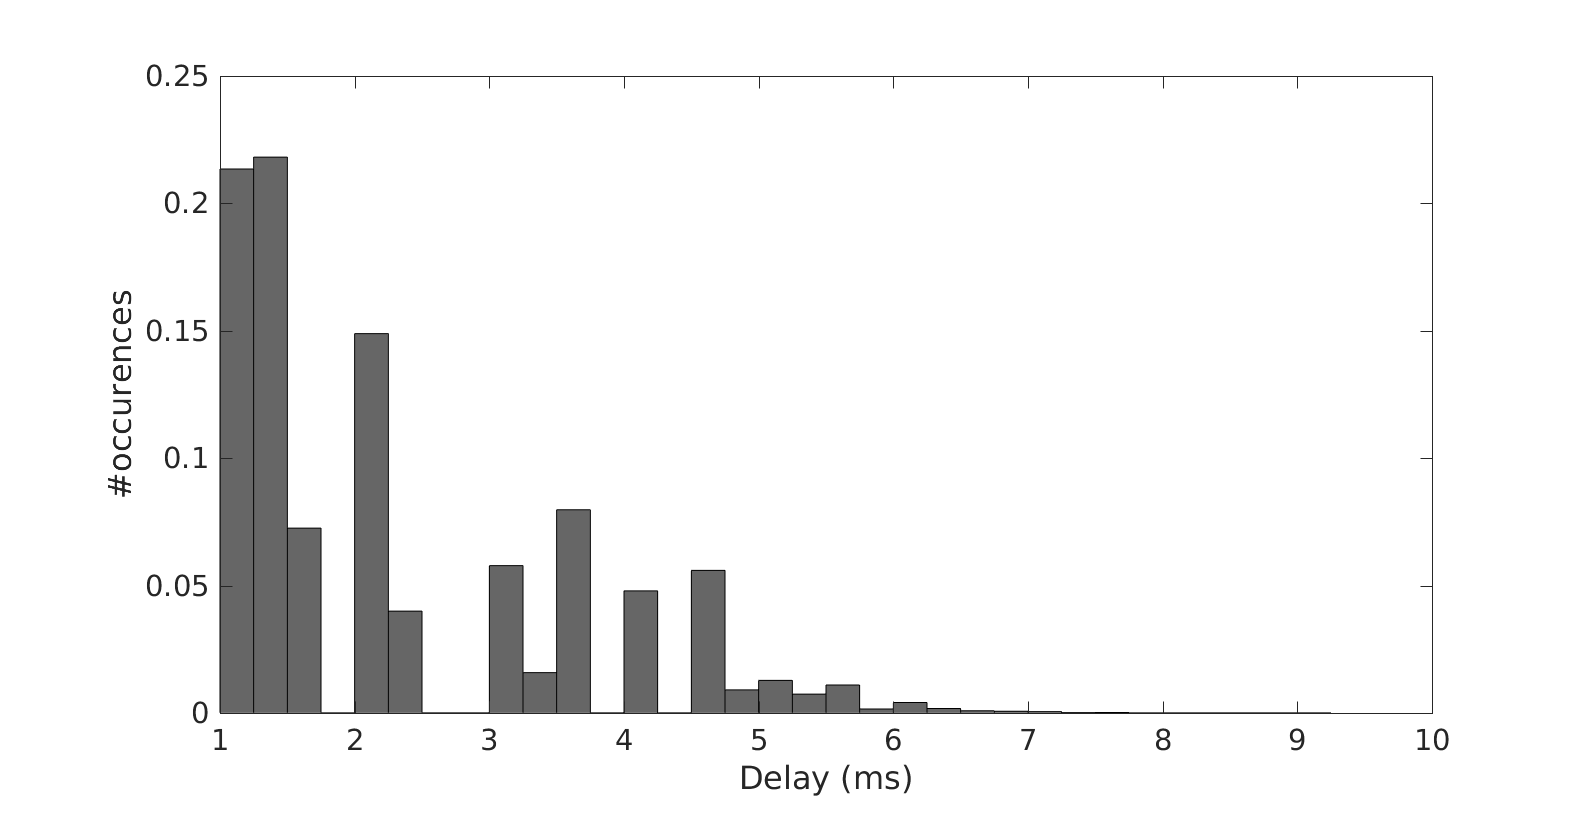
\includegraphics[width=0.6\textwidth]{fig/DelayDistributionForest} }
 \label{fig:connection_delay_distrbution_forest}
\end{figure}
 \FloatBarrier

We first stimulate the forest with model parameters at $\Sigma$ with a uniform background stimulus. 
We observe large-scale traveling waves including spiral and spreading waves.
\begin{figure}[!htb]
 \caption{ Wave patterns spreading in the X-Y plane of a forest of minicolumns. 
           The system is a forest of 50x50 minicolumns, each minicolumn is 2x2x10. 
           Model parameters are at $\Sigma$ and the system has absorbing boundary conditions. 
           }
   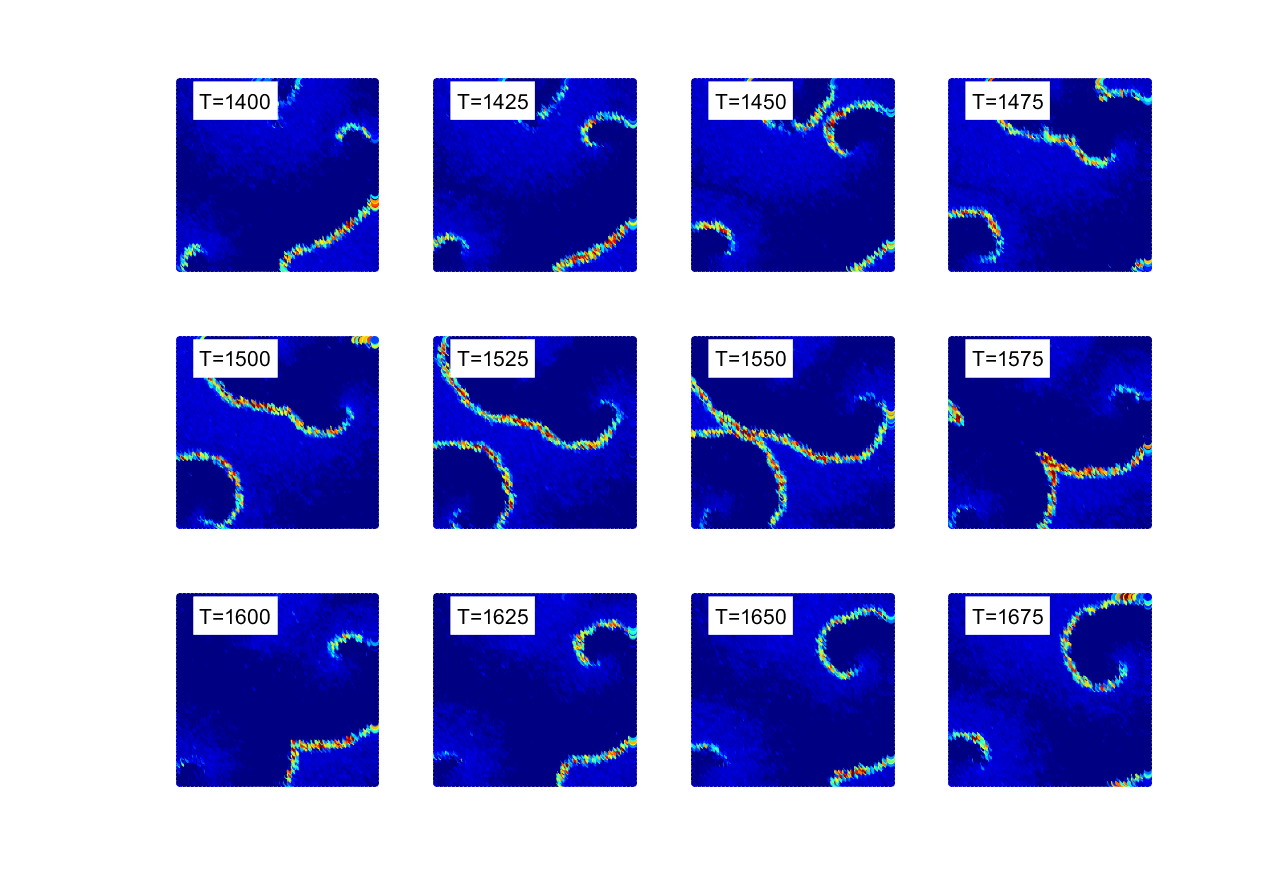
\includegraphics[width=\textwidth]{fig/Forest_SpreadingWaves_K10_Sep2p5}
   \label{fig:ForestSpiralWaves}
\end{figure}
\FloatBarrier

The forest of minicolumns supports traveling waves even though the inter-column connectivity is relatively sparse.
The higher connectivity within the minicolumns support extended firing activity that is able to stimulate adjacent minicolumns.
The spatio-temporal patterns in the simulation continue to evolve and do not settle into a repeating pattern.

\begin{figure}[!htb]
 \caption{Spike timing characterization of the forest waves seen in figure \ref{fig:ForestSpiralWaves}.
          a) The spike raster from a small number of neurons show regular spike events that correspond to passing waves, with neurons spiking several times as the wave passes.
          b) The log histogram of all inter-spike intervals does not show a prominent single peak, indicating that the system did not settle into a repeating pattern. 
          c) The distribution of the coefficient of variation showing that the neuron firing times are irregular.
          d) The average correlation coefficient as a function of distance shows that the firing times of nearby neurons are highly correlated due to the wave structure.
          } 
     \subfloat[][]{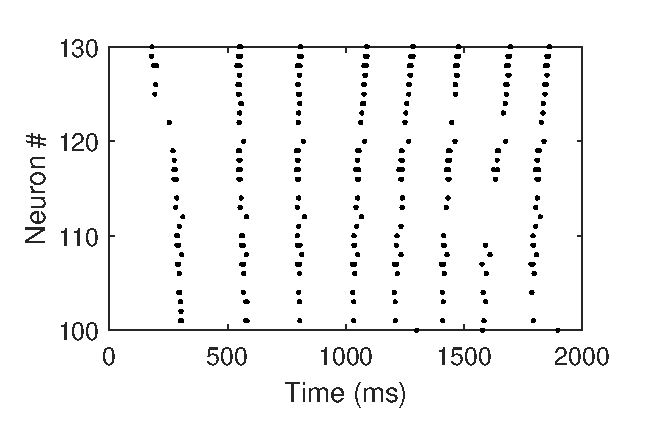
\includegraphics[width=0.48\textwidth]{fig/ForestSpiralWaves_CorrelationRasterPlot} }
     \subfloat[][]{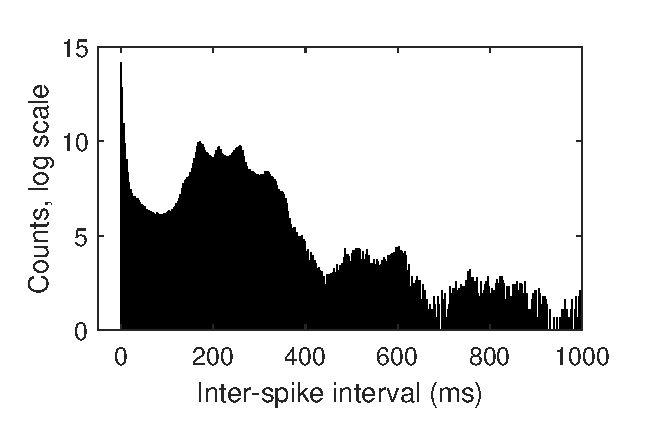
\includegraphics[width=0.48\textwidth]{fig/ForestSpiralWaves_ISI} }
     \subfloat[][]{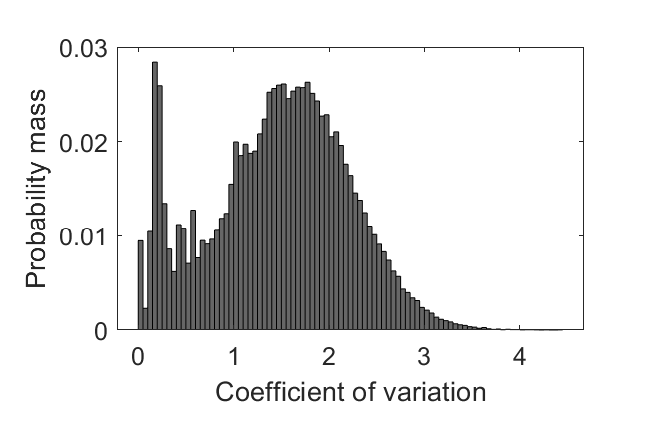
\includegraphics[width=0.48\textwidth]{fig/ForestSpiralWaves_CVDist} }
     \subfloat[][]{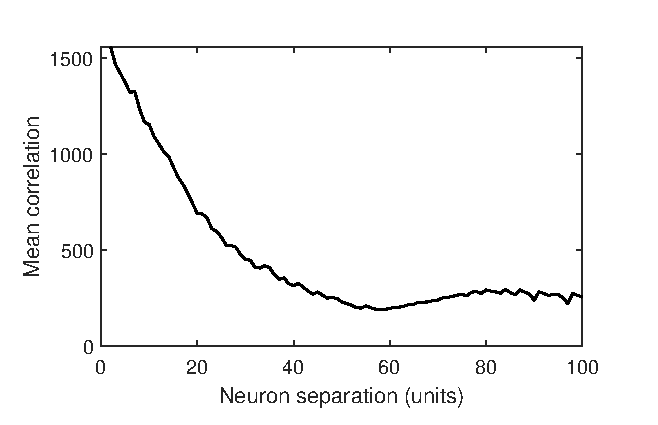
\includegraphics[width=0.48\textwidth]{fig/ForestSpiralWaves_CorrelationCoefficient} }
 \label{fig:ForestSpiralWave_SpikeTiming}
\end{figure}


We now increase K from 10 to 14, expecting to see the spiral waves disappear based on our observations in the quasi 2-D sheet.
We  observe two-dimensional traveling wave patterns in the forest when viewing the X-Y plane from above (Figure \ref{fig:ForestSpreadingWaves}).
We again observe a repeating spatio-temporal pattern with a repetition rate of about $200~ms$.

\begin{figure}[!htb]
 \caption{ Wave patterns spreading in the X-Y plane of a forest of minicolumns. 
           The system is a forest of 50x50 minicolumns, each minicolumn is 2x2x10. 
           Connection strength is increased to $K=14$ and the system has absorbing boundary conditions. 
           }
   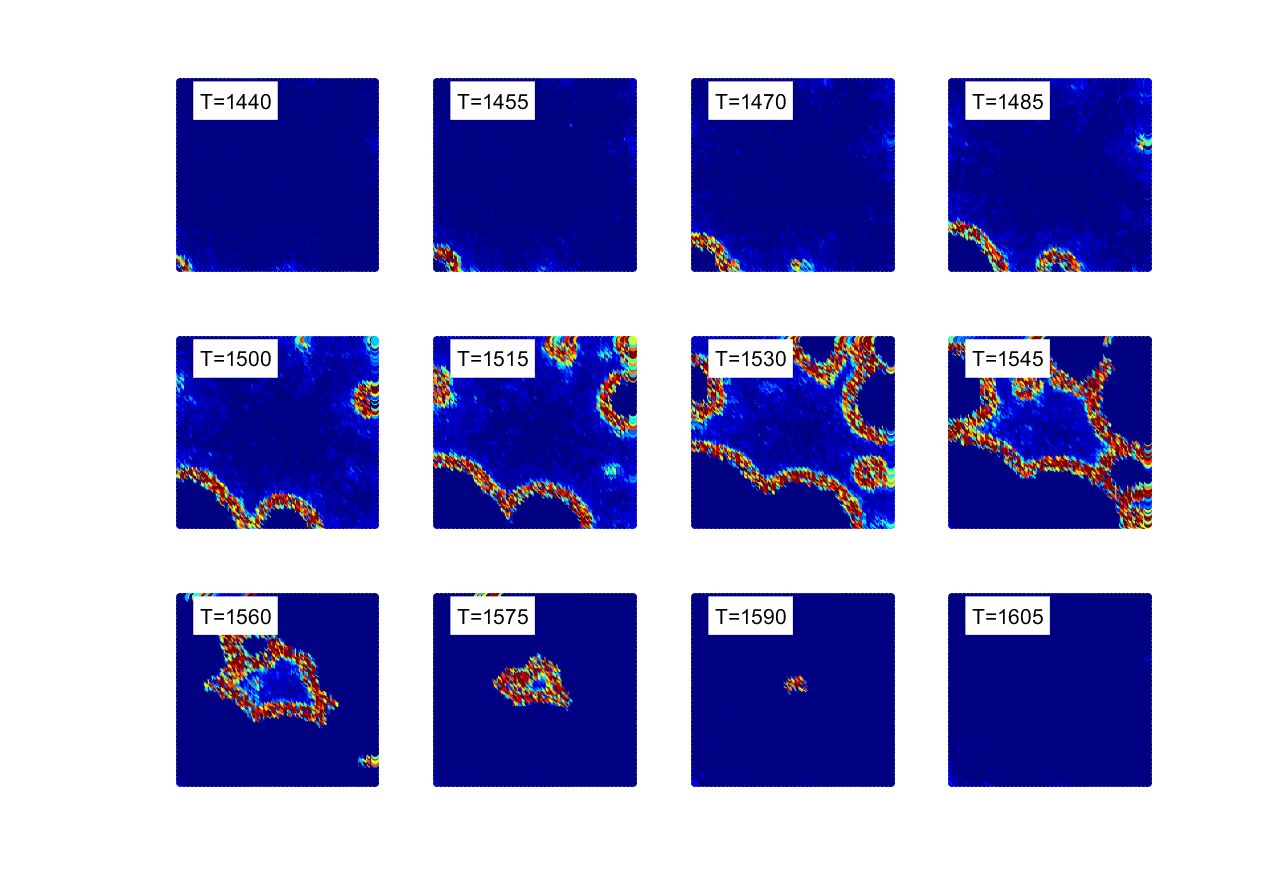
\includegraphics[width=\textwidth]{fig/Forest_SpreadingWaves_K14_Sep2p5}
   \label{fig:ForestSpreadingWaves}
\end{figure}
\FloatBarrier

In a quasi-2D system we observed repeating spatiotemporal patterns that created highly regular firing rates in the individual neurons.
In our forest of minicolumns we still observe a repetitive large-scale spatiotemporal structure, but the firing activity of the individual neurons shows more variation.
Rather than firing once or twice when a wave passes, the individual neurons fire several times in an irregular pattern 
driven by the activity within the local minicolumn (Figure \ref{fig:ForestSpreadingWave_SpikeTiming}).
Plotting the inter-spike interval histogram on a log scale reveals that the most prevalent ISIs are very short, 
indicating individual neurons firing multiple times in close succession (Figure \ref{fig:ForestSpreadingWave_SpikeTiming}b).
We still see a peak in the vicinity of $200~ms$ indicating the spatio-temporal repetition rate.
We also see smaller peaks near multiples of $200~ms$ indicating that some neurons were not triggered by every passing wave.
\begin{figure}[!htb]
 \caption{Spike timing characterization of the forest waves seen in figure \ref{fig:ForestSpreadingWaves}.
          a) The spike raster from a small number of neurons show regular spike events that correspond to passing waves, with neurons spiking several times as the wave passes.
          b) The log histogram of all inter-spike intervals shows a repetition period of $200~ms$ due to the passing waves, 
             with peaks at longer ISI because not all neurons fire when a wave passes. 
          c) The distribution of the coefficient of variation showing that the neuron firing times are irregular.
          d) The average correlation coefficient as a function of distance shows that the firing times of nearby neurons are highly correlated due to the wave structure.
          } 
     \subfloat[][]{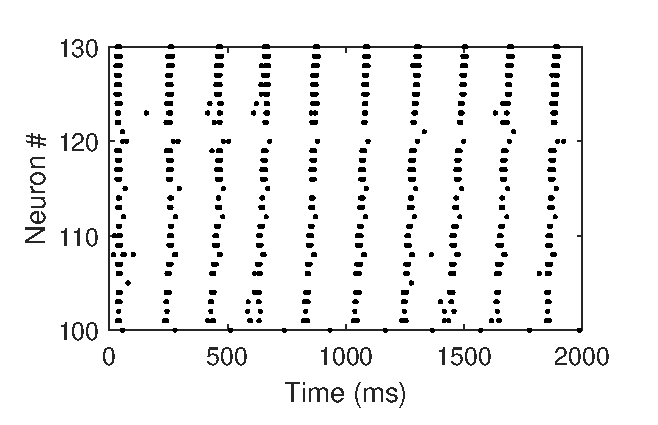
\includegraphics[width=0.48\textwidth]{fig/ForestSpreadingWaves_CorrelationRasterPlot} }
     \subfloat[][]{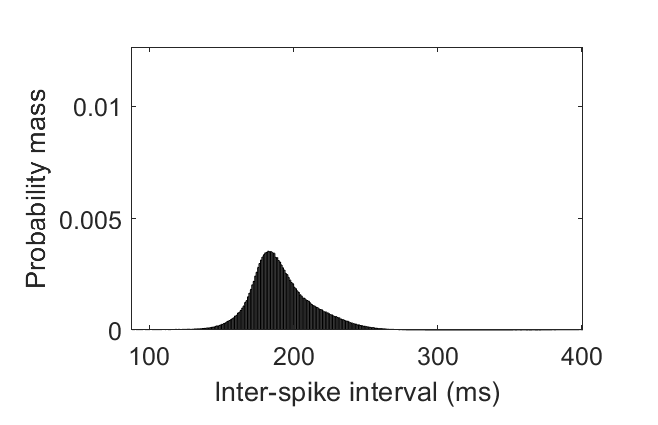
\includegraphics[width=0.48\textwidth]{fig/ForestSpreadingWaves_ISI} }
     \subfloat[][]{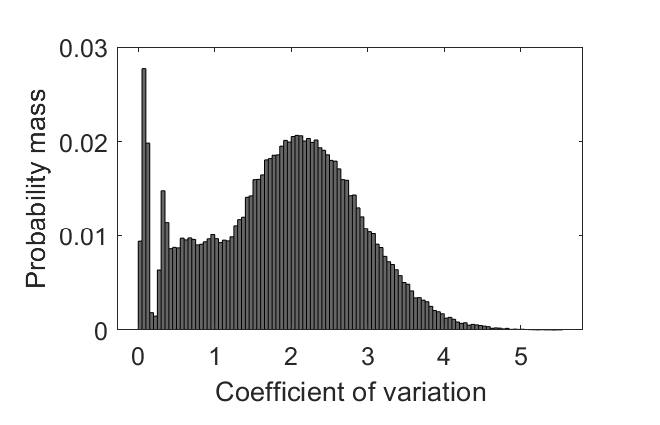
\includegraphics[width=0.48\textwidth]{fig/ForestSpreadingWaves_CVDist} }
     \subfloat[][]{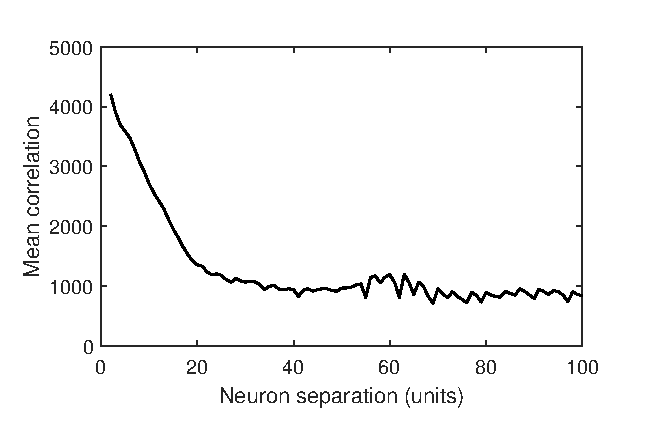
\includegraphics[width=0.48\textwidth]{fig/ForestSpreadingWaves_CorrelationCoefficient} }
 \label{fig:ForestSpreadingWave_SpikeTiming}
\end{figure}
 \FloatBarrier
 

\endinput
%%
%% End of file `example-1.tex'.
